% !TEX encoding = UTF-8 Unicode
% !TEX spellcheck = en_US

\documentclass[a4paper,twoside]{article}
\usepackage[T1]{fontenc}
\usepackage[utf8]{inputenc}
\usepackage{epsfig}
\usepackage{subcaption}
\usepackage{calc}
\usepackage{amssymb}
\usepackage{amstext}
\usepackage{amsmath}
\usepackage{amsthm}
\usepackage{multicol}
\usepackage{pslatex}
\usepackage{apalike}
\usepackage{paralist} % for compactitem
\usepackage{bm}
\usepackage{color}
\usepackage{nicefrac}
\usepackage{siunitx}
\usepackage{url}
\graphicspath{{./figures/}}
\newcommand{\ks}[1]{{(\mathrm{CS})}_{#1}}
\newcommand{\transp}[0]{{\mathrm{T}}}
\newcommand{\rotmat}[2]{{{ }^{#1}\boldsymbol{R}}_{#2}}
\DeclareMathOperator*{\argmin}{argmin}
\usepackage{SCITEPRESS}     % Please add other packages that you may need BEFORE the SCITEPRESS.sty package.
\hyphenation{Rei-ter}
\hyphenation{off-line}

\begin{document}

\title{Singularity Avoidance of Task-Redundant Robots in Pointing Tasks: \\On Nullspace Projection and Cardan Angles as Orientation Coordinates}

% TODO: Leave empty upon initial submission for double-blind review
\author{\authorname{Moritz Schappler\sup{1}\orcidAuthor{0000-0001-7952-7363}
and Tobias Ortmaier\sup{1}\orcidAuthor{0000-0003-1644-3685}}
\affiliation{\sup{1}Institute of Mechatronic Systems, Leibniz University Hannover, An der Universität 2, 30823 Garbsen, Germany}
\email{\{moritz.schappler, tobias.ortmaier\}@imes.uni-hannover.de}}


\keywords{Singularity Avoidance, Nullspace Motion, Task Redundancy, Parallel Robots, Euler Angles, Cardan Angles.}

\abstract{
Robot manipulators are often deployed in tool-symmetric tasks, which only requires defining end effector position and pointing direction.
In this case six-axis serial industrial robots and full-mobility (spatial) parallel robots have  one degree of task redundancy.
Using Cardan angles as orientation coordinates, a unified formulation of the position-level and second-order inverse kinematics problem is set up for both robot types.
An efficient scheme for difference-quotient approximation of gradients of performance criteria for projection into the task redundancy's nullspace is presented.
The simulation example of a hexapod robot shows that avoiding and exiting parallel robot singularities of type II is possible with the nullspace of all joints.
The nullspace controller scheme can be used in offline trajectory optimization and in online motion generation.
}

\onecolumn \maketitle \normalsize \setcounter{footnote}{0} \vfill

\section{\uppercase{Introduction and State of the Art}}
\label{sec:introduction}

Robot manipulators have been a subject of research for decades.
Still more complex parallel kinematic machines (parallel robots), and more complex problems arise, such as mastering singularities and motion in high-dimensional spaces.
Due to their complexity, these problems can only be solved with profound algorithms and by the help of information technology.

The optimization of robots performing tasks with axis-symmetric tools like arc welding \cite{HuoBar2008}, drilling \cite{GuoDonKe2015} or milling \cite{MousaviGagBouRay2018} has gained increasing attention in research and industry over the last years.
Due to their workspace, serial robots are predestinated for welding tasks but also for drilling tasks e.g. in the aircraft industry.
For machining tasks parallel robots are favorable due to their higher stiffness than serial kinematic machine tools or serial robot arm manipulators.

Serial industrial robots as well as the hexapod parallel robot often used for machining tasks have six degrees of freedom (DoF) in the operational space and in the (actuation) joint space.
They do not have \emph{intrinsic redundancy} (for serial robots) or \emph{kinematic or actuation redundancy} (in the case of parallel robots).
A \emph{task (or functional) redundancy} of degree one exists, if the six-DoF robot is used in an axis-symmetric task (requiring only five DoF).
For a definition of the redundancy see \cite{HuoBar2008} or \cite{LegerAng2016} for serial robots and \cite{GosselinSch2018} for parallel robots.

The redundancy allows defining a nullspace and performing a pose optimization using gradient projection into that nullspace.
This method is very efficient and already well-established for \emph{kinematic} redundancy \cite{NakamuraHanYos1987,ChiaveriniOriWal2008,LilloChiAnt2019}.
The redundancy of a rotational end effector DoF requires the adaption of the inverse kinematics problem (IKP) to account for the nonlinearity of rotation.
Further, the IKP can be distinguished between position level and velocity level or higher differential order.
Several geometric approaches for the IKP of \emph{task}-redundant robots have been investigated, such as 
\begin{compactitem}
\item twist decomposition \cite{HuoBar2008},
\item orthogonal decomposition of the task space \cite{LegerAng2016,CorinaldiAngCal2016},
\item reciprocal Euler angles
 \cite{SchapplerTapOrt2019},
\item separation of joint coordinates in redundant and non-redundant on position level \cite{Ozgoren2013} or on velocity level \cite{ReiterMueGat2018},
\item expressing the end effector angular velocity in the local frame and removing the last component \cite{Zlajpah2017,ReiterMueGat2018} corresponding to the redundant coordinate.
\end{compactitem}
\pagebreak

The alternative to the modified inverse kinematics (IK) formulations above is a full formulation of the IK (ignoring task redundancy).
Then, a subsequent optimization of the redundant task space coordinate is necessary, as performed by \cite{ZhuQuCaoYan2013}, \cite{GuoDonKe2015} and \cite{MousaviGagBouRay2018} for serial robots.
Especially for parallel robots this approach was previously pursued combined with
\begin{compactitem}
\item interval analysis \cite{MerletPerDan2000}, 
\item an iterative solution using linear or quadratic programming \cite{OenWan2007},
\item discrete switching patterns of the redundant coordinate in rest positions \cite{KotlarskiDoHeiOrt2010},
\item iterations of small-angle perturbations of the redundant coordinate \cite{GaoCheGaoXia2019}.
\end{compactitem}

In special variations of the milling task using parallel kinematic machines (PKM), more than one rotational coordinate can be treated as redundant.
Examples are end milling \cite{ShawChe2001} or milling with a spherical cutter \cite{SmirnovPlyMir2013}.

The overview already shows that gradient-based local optimization approaches are more widely used in serial robotics than in parallel robotics, where global optimizations dominate.
A promising strategy is the combination of local and global approaches, e.g. by using differential dynamic programming \cite{SantosSil2017}.


Only in recent publications, gradient-based optimization with nullspace projection is performed for parallel robots, with focus on kinematic redundancy by \cite{GosselinSch2016} and \cite{SantosSil2017} and on task redundancy by \cite{AgarwalNasBan2016}.
The main effort is put on the kinematic and actuation redundancy, as can be seen in the extensive reviews on parallel robot redundancy \cite{LucesMilBen2017} and \cite{GosselinSch2018}, where task redundancy is not even mentioned.

Redundancy is exploited to improve performance criteria of the robot manipulators, such as joint limits \cite{HuoBar2008,ZhuQuCaoYan2013} or milling process stability \cite{MousaviGagBouRay2018}.
Singularity avoidance is implemented by criteria such as 
\begin{compactitem}
\item the distance in the joint space to the configuration that first exceeded a parameter of singularity \cite{HuoBar2008},
\item the squared condition number \cite{ZhuQuCaoYan2013,LegerAng2016,CorinaldiAngCal2016} via the Frobenius norm relation \cite{Merlet2006a},
\item the condition number of the PKM forward kinematics Jacobian \cite{GosselinSch2016}, % term "geometric matrix of forward kinematics" would be more appropriate, but is not used for the sake of simplicity
\item the consideration of all singular values of the Jacobian \cite{SantosSil2017},
\item the homogenized pose error as a measure for accuracy and singularities \cite{KotlarskiDoHeiOrt2010},
\item the Jacobian's determinant \cite{AgarwalNasBan2016}.
\end{compactitem}

Although the physical meaning of the manipulator Jacobian's condition number is questionable, cf. \cite{KotlarskiDoHeiOrt2010}, using it as a measure for singularity avoidance is well established and can be justified, even without homogenization of units, cf. \cite{Merlet2006a}.
Especially for parallel robots singularities %of type II, see \cite{Merlet2006a},
can be located anywhere in the workspace and avoiding them in offline trajectory planning and online trajectory execution is paramount, cf. \cite{LucesMilBen2017,GosselinSch2018}.

The work from \cite{AgarwalNasBan2016} presents a promising approach to tackle the problem of singularity avoidance for parallel robots using gradient projection in the nullspace of task redundancy.
However, open points remain, regarding the feedback loop design of the nullspace motion and an extension to spatial robots regarding the nonlinearity of rotation.
%
These points will be encountered in this paper %by extending the work from  \cite{AgarwalNasBan2016} 
by a consideration of Cardan angles as end effector coordinates, as in \cite{SchapplerTapOrt2019}, by considering a second-order nullspace motion, cf. \cite{ReiterMueGat2018} and by incorporating aspects of control design from \cite{DeLucaOriSic1992}, where this problem was already approached for serial robots.
%
To summarize, the contributions of this paper are
\begin{compactitem}
\item a formulation of the differential inverse kinematics problem for one-DoF task redundancy using Cardan angles for end effector orientation,
\item a numeric scheme for simplification of the computation of gradients of performance criteria in the nullspace projection using difference quotients,
\item unifying the scheme for serial and parallel robots,
\item and exemplary simulative studies on offline trajectory planning with singularity avoidance.
\end{compactitem}

The remainder of the paper is structured as follows.
After a remark on task coordinates in section~\ref{sec:coord},
the kinematics model and nullspace motion is laid out in section~\ref{sec:serrob} for serial robots and in section~\ref{sec:parrob} for parallel robots.
Considerations on the control loop design and remarks on convergence are given in section~\ref{sec:control_loop} and the scheme is validated in section~\ref{sec:casestudy} at the example of pose optimization 
and trajectory tracking 
of a six-DoF parallel robot.
Section~\ref{sec:conclusion} concludes the paper.

\section{\uppercase{On Task Coordinates}}
\label{sec:coord}

In the following, the six \emph{operational space coordinates}, i.e. the position and orientation of a robot's end effector in the Cartesian space, are expressed with the vector $\bm{x}=(r_x,r_y,r_z,\varphi_x,\varphi_y,\varphi_z)^\transp$.
Unlike for the unambiguous position part $\bm{r}$, a suitable representation of rotation has to be chosen for the orientation part $\bm{\varphi}$.

For tasks with rotational symmetry given in section~\ref{sec:introduction}, a selection of the Euler angle convention is suitable, where the last of the three (intrinsic) elementary rotations is defined around the tool axis.
The Cardan angles (or $X$-$Y$'-$Z$'' Euler angles) are especially practical and intuitive, since the tool axis in robotics is by convention the $\bm{z}_E$-axis. 
The end effector's rotation matrix w.r.t. the base frame is defined by $\rotmat{0}{E}(\bm{x})=\bm{R}_x(\varphi_x) \bm{R}_y(\varphi_y) \bm{R}_z(\varphi_z)$ using the basic rotation matrices.
The angle convention established in tool machines on the contrary follows the extrinsic $X$-$Y$-$Z$ Euler angles convention for expressing orientation, which corresponds to the intrinsic $Z$\nobreakdash-$Y$'\nobreakdash-$X$'' convention.
The rotation axes are termed ``A, B and C'' (corresponding to ``X, Y and Z'' translation), \cite{SmirnovPlyMir2013}.
The term ``Euler angles'' is used for generalization, also including Tait-Bryan (and Cardan) angles and is not limited to proper Euler angles.
Representing orientation with Euler angles can introduce mathematical singularities corresponding to a gimbal lock.
For Cardan angles this only occurs for $\varphi_y{=}\pm$\SI{90}{\degree}, which is not relevant for most tasks and e.g. technically not possible for most parallel robots and therefore out of this paper's scope.

The \emph{task space coordinates} of pointing tasks are defined as ${\bm{y}=(r_x,r_y,r_z,\varphi_x,\varphi_y)^\transp}$.
Due to the rotational symmetry of the robot tool and the chosen representation of rotation, the last operational space coordinate $\varphi_z$ corresponds to a rotation of the robot end effector around the tool axis and can be selected arbitrarily in the regarded case of task redundancy.

\section{\uppercase{Serial-Link Robots}}
\label{sec:serrob}

Redundancy resolution for serial robots has been widely researched, cf. \cite{ChiaveriniOriWal2008}, but the case of task redundancy is only implicitly included in the fundamental works.
%
In the following, section~\ref{sec:ikp_serrob} clarifies some foundations e.g. from \cite{ChiaveriniOriWal2008} regarding task redundancy and section~\ref{sec:nullspace_serrob} introduces new aspects on the computation of the nullspace in task redundancy.

\subsection{Inverse Kinematics Model}
\label{sec:ikp_serrob}

% forward kinematics

The forward kinematics problem relates the $n_{\bm{q}}$ joint space coordinates $\bm{q}$ with the operational space by
\begin{equation}
\bm{x}=\left[\bm{x}_{\mathrm{t}}^\transp,\,\bm{x}_{\mathrm{r}}^\transp\right]^\transp
=
\left[\bm{r}_E^\transp(\bm{q}),\,\bm{\varphi}_{XYZ}^\transp(\rotmat{0}{E}(\bm{q}))\right]^\transp.
\label{eq:ser_fkin}
\end{equation}
% full residual
The non-redundant inverse kinematics problem (IKP) can be expressed by an implicit residual in $\mathbb{R}^6$
\begin{equation}
\bm{\Phi}(\bm{q},\bm{x})
=
\begin{bmatrix}
\bm{\Phi}_\mathrm{t} \\
\bm{\Phi}_\mathrm{r}
\end{bmatrix}
=
\begin{bmatrix}
-\bm{x}_{\mathrm{t}}+\bm{r}_E(\bm{q}) \\
\bm{\theta}\left(\rotmat{0}{E}^\transp (\bm{x}_{\mathrm{r}})\rotmat{0}{E}(\bm{q})\right)
\end{bmatrix}
=
\bm{0} %\in \mathbb{R}^6,
\label{eq:ser_residual_full}
\end{equation}
with arbitrary convention $\bm{\theta}$, which can be solved numerically using the Newton-Raphson algorithm.
% reduced residual 
In the case of task redundancy, a reduced residual
\begin{equation}
\bm{\Psi}(\bm{q},\bm{y})=\bm{0} \in \mathbb{R}^5 \quad \mathrm{with~rotational~part} 
\label{eq:ser_residual_red}
\end{equation}
\begin{equation}
\bm{\Psi}_\mathrm{r}
=
{\begin{bmatrix}
	0 & 1 & 0  \\ 
	0 & 0 & 1
	\end{bmatrix}}
\bm{\theta}_{ZYX}\left(\rotmat{0}{E}^\transp (\bm{x}_{\mathrm{r}})\rotmat{0}{E}(\bm{q})\right)
 \in \mathbb{R}^2
\label{eq:ser_residual_red_rot}
\end{equation}
is needed, which can be set up by using the Euler angles $\bm{\theta}$ of the rotation matrix between desired pose $\bm{x}$ and actual pose $\bm{x}(\bm{q})$.
The angle convention in $\bm{\Psi}$ has to be reciprocal (i.e. $Z$-$Y$'-$X$'') to the one used for the end effector pose $\bm{x}$, as derived in \cite{SchapplerTapOrt2019}.
The redundant coordinate $\varphi_z$ has no effect.

Using a task-redundant robot with $n_{\bm{q}} \geq 6$ allows to optimize additional objective functions $h(\bm{q})$ using nullspace projection in the iterative solution by
\begin{equation}
\bm{q}_{\mathrm{opt}}=\argmin_{\bm{q}}(h(\bm{q}))\quad\mathrm{s.t.}\quad \bm{\Psi}(\bm{q},\bm{y})=\bm{0}.
\end{equation}

The iterative solution in the step $k$ is obtained with the Moore-Penrose pseudo-inverse by
\begin{equation}
\bm{q}^{k+1}=\bm{q}^{k} - 
=
\bm{\Psi}_{\partial \bm{q}}^{\#}\bm{\Psi}+(\bm{I}_{n_{\bm{q}}}-\bm{\Psi}_{\partial \bm{q}}^{\#}\bm{\Psi}_{\partial \bm{q}}) (-h_{\partial \bm{q}}^\transp),
\label{eq:ser_position_ik}
\end{equation}
where the index $\partial \bm{q}$ denotes the derivative of the symbol w.r.t. $\bm{q}$, \# the pseudo-inverse, $\bm{I}_{n_{\bm{q}}}$ the identity matrix of appropriate dimension $n_{\bm{q}}$ and the dependency on $\bm{q}^{k}$ and $\bm{y}$ is omitted for the sake of brevity.
The notation will be kept throughout the paper.

% differential kinematics in operational space
Using this allows to optimize the robot for one specific pose, e.g. for drilling tasks, where the feed motion is negligible regarding the robot's dimension.
To obtain a continuous trajectory, e.g. for milling tasks, the forward differential kinematics 
\begin{equation}
\dot{\bm{x}}=\bm{J}_{\bm{x}} \dot{\bm{q}}\quad\mathrm{and}\quad \ddot{\bm{x}}=\dot{\bm{J}}_{\bm{x}} \dot{\bm{q}} + \bm{J}_{\bm{x}} \ddot{\bm{q}}
\label{eq:ser_diff_kin}
\end{equation}
are used.
The matrix $\bm{J}_{\bm{x}}$ is known as the analytic Jacobian.
The geometric Jacobian on the contrary relates angular velocities in the base frame instead of time derivatives of the Euler angles to the joint velocities.

The transfer from operational space to task space is performed by removing the last row of (\ref{eq:ser_diff_kin}) with $\bm{y}=\bm{P}_{\bm{y}} \bm{x}$ and $\bm{J}_{\bm{y}} = \bm{P}_{\bm{y}} \bm{J}_{\bm{x}}$. %, where
%The indices $\bm{x}$ and $\bm{y}$ denote the operational and task space.
The matrices $\bm{J}_{\bm{y}}$ and $\bm{\Psi}_{\partial \bm{q}}$ are not identical due to the nonlinearity of rotation in $\mathrm{SE(3)}$.
The task space inverse differential kinematics are obtained by the pseudo-inverse solution
\begin{equation}
\ddot{\bm{q}}
=\ddot{\bm{q}}_\mathrm{T}+\ddot{\bm{q}}_\mathrm{N}
= \bm{J}_{\bm{y}}^{\#}(\ddot{\bm{y}} - \dot{\bm{J}}_{\bm{y}} \dot{\bm{q}}) + (\bm{I}_{n_{\bm{q}}}-\bm{J}_{\bm{y}}^{\#}\bm{J}_{\bm{y}}) \bm{v}.
\label{eq:ser_accel_ik}
\end{equation}
Again as in (\ref{eq:ser_position_ik}), nullspace projection of arbitrary vectors $\bm{v}$ can be performed.
The vector may be chosen as $\bm{v}=-h_{\partial \bm{q}}^\transp$ or as discussed in section~\ref{sec:control_loop}.


\subsection{Task Redundancy and Nullspace}
\label{sec:nullspace_serrob}

Objective functions $h(\bm{q})$ can be defined analytically or numerically.
The former is not possible or feasible for all functions.
For the latter a method for the efficient derivation of the gradient $h_{\partial \bm{q}}$ will be presented and discussed for several cases.
%One possible objective function can be the condition number of the manipulator's Jacobian matrix $h(\bm{q})=\mathrm{cond}(\bm{J}_{\bm{x}}(\bm{q}))$.

\subsubsection{General Case}
\label{sec:nullspace_serrob_general}

The general case is not limited to task redundancy and can be used in the position-level inverse kinematics problem (\ref{eq:ser_position_ik}) for $\lVert\bm{\Psi}\rVert \not\approx 0$.
A difference quotient is calculated for a small increment $\Delta q_i$ of all joints by
%
\begin{equation}
h_{\partial q_i} \approx (h(\bm{q}+\Delta \bm{q}) - h(\bm{q}))/\Delta q_i,
\label{eq:ser_diffquot_general}
\end{equation}
%
where $\Delta q_j = 0$ with $j \neq i$ in $\Delta \bm{q}$. %  and $\Delta q_i$is chosen sufficiently small.
This requires $n_{\bm{q}}{+}1$ evaluations of the objective function $h(\bm{q})$ in each iteration of (\ref{eq:ser_position_ik}) or each discrete trajectory sample of (\ref{eq:ser_accel_ik}).
This is e.g. mentioned in \cite{LilloChiAnt2019}, but is probably used in many implementations.

\subsubsection{Task Redundancy of Degree One}

In the case of task redundancy with $n_{\bm{q}}{-}\mathrm{dim}(\bm{y})=1$, the nullspace projection can be exploited to simplify the computation.
The assumption is that $\lVert\bm{\Psi}\rVert \approx 0$, which is always the case in the differential inverse kinematics (\ref{eq:ser_accel_ik}).
In the position-level IKP (\ref{eq:ser_position_ik}) convergence of the task or an already valid initial value $\bm{q}^{0}$ is required.
Writing $\bm{q}:=\bm{q}(\bm{x})$ leads to
\begin{equation}
\frac{\partial h}{\partial \bm{x}} = \frac{\partial h}{\partial \bm{q}} \frac{\partial \bm{q}}{\partial \bm{x}}
\quad \mathrm{or} \quad 
\frac{\partial h}{\partial \bm{q}} = \frac{\partial h}{\partial \bm{x}} \frac{\partial \bm{x}}{\partial \bm{q}}.
\label{eq:ser_gradient_opspace}
\end{equation}
The latter expression can be divided into the single operational space coordinates via
\begin{equation}
\frac{\partial h}{\partial \bm{q}} =
\frac{\partial h}{\partial r_x} \frac{\partial r_x}{\partial \bm{q}}
+
\frac{\partial h}{\partial r_y} \frac{\partial r_y}{\partial \bm{q}}
+ \hdots +
\frac{\partial h}{\partial \varphi_z} \frac{\partial \varphi_z}{\partial \bm{q}}.
\label{eq:ser_gradient_algebraic_conversion}
\end{equation}
The nullspace projector included in (\ref{eq:ser_position_ik}) or (\ref{eq:ser_accel_ik}) is
\begin{equation}
\bm{N}
= \bm{I}_{n_{\bm{q}}}-\bm{J}_{\bm{y}}^{\#}\bm{J}_{\bm{y}}
= \bm{I}_{n_{\bm{q}}}-\bm{\Psi}_{\partial \bm{q}}^{\#}\bm{\Psi}_{\partial \bm{q}}
\enspace \mathrm{for}\enspace \lVert\bm{\Psi}\rVert = 0.
\label{eq:ser_nullspace_projector}
\end{equation}
Since the nullspace is defined as a rotation within the $\varphi_z$ coordinate, the projector eliminates the other terms
\begin{equation}
\bm{N}\left(\frac{\partial h}{\partial r_x} \frac{\partial r_x}{\partial \bm{q}}\right)^\transp \hspace{-0.5mm}=\bm{0}, % shift equation sign to the left (transpose takes too much space)
\enskip \hdots, \enskip
\bm{N}\left(\frac{\partial h}{\partial \varphi_y} \frac{\partial \varphi_y}{\partial \bm{q}}\right)^\transp \hspace{-0.5mm}=\bm{0}.
\label{eq:serrob_nullspace_elim}
\end{equation}
Therefore the gradient in the case of one-DoF task redundancy can be simplified to
\begin{equation}
h_{\partial \bm{q}}^{*} 
= 
\frac{\partial h}{\partial \varphi_z} \frac{\partial \varphi_z}{\partial \bm{q}},
\label{eq:serrob_nullspace_phiz}
\end{equation}
where the last term is the last row of the Jacobian $\bm{J}_{\bm{x}}$.
The asterisk denotes the simplified calculation of the gradient which follows the relations
\begin{equation}
\bm{N} (h_{\partial \bm{q}}^{*})^\transp = \bm{N} (h_{\partial \bm{q}})^\transp
\quad\mathrm{and}\quad
h_{\partial \bm{q}}^{*} \neq h_{\partial \bm{q}}.
\label{eq:serrob_nullspaceproj_equivalence}
\end{equation}
Using a small increment of the redundant coordinate $\Delta \bm{x}=(\bm{0}^\transp,\Delta  \varphi_z)^\transp$, the first term can be determined numerically via the difference quotient

%Approximation of differential
\begin{equation}
(\partial h / \partial \varphi_z) \approx (h(\bm{q}+\bm{J}_{\bm{x}}^{-1}\Delta \bm{x}) - h(\bm{q}))/\Delta \varphi_z.
\label{eq:serrob_nullspace_h_phiz}
\end{equation}
This only requires two numeric evaluations of $h(\bm{q})$ which can be highly beneficial for computationally expensive objectives such as collision avoidance or singularity avoidance.
The approach of simulating a $\Delta \varphi_z$ can be regarded similar to the principle of small-angle perturbation of \cite{GaoCheGaoXia2019}, where a global instead of local optimization is performed.


\section{\uppercase{Parallel Robots}}
\label{sec:parrob}

% General case: parallel robot model with all active, passive joint coordinates,
The inverse kinematics of task redundant parallel robots can be approached similarly as serial robots.
A a parallel robot consists of $m$ kinematic chains connecting a base link with a moving platform.
Following e.g. \cite{Merlet2006a}, the joint space $\bm{q}$ now also contains passive joints (here also including the platform coupling joints).
Active joint coordinates are included in this formulation and are also denoted by $\bm{\theta}$.
Further, the platform pose can be expressed by the operational space coordinate $\bm{x}$ which can also be used as a minimal coordinate of the robot.

In the following, section~\ref{sec:ikp_parrob} again applies approaches from literature, e.g. \cite{Merlet2006a,ChiaveriniOriWal2008} to task redundancy and section~\ref{sec:nullspace_parrob} discusses projection in the nullspace.

\subsection{Inverse Kinematics Model}
\label{sec:ikp_parrob}

% Definition of full kinematic constraints similar to serial robot

To solve the IKP for parallel robots, similar to (\ref{eq:ser_residual_full}) and (\ref{eq:ser_residual_red}) for serial robots, the full and reduced kinematic constraints $\bm{\Phi}(\bm{q},\bm{x}){\in}\mathbb{R}^{6m}$ and $\bm{\Psi}(\bm{q},\bm{y}){\in}\mathbb{R}^{6m-1}$ are defined.
The latter can be obtained in the minimal form only dependent on the task space coordinate $\bm{y}$ by using reciprocal Euler angles for the orientation constraints of the first leg chain like in (\ref{eq:ser_residual_red_rot}).
The constraints of other (following) legs are defined relative to the first (leading) leg, e.g. as vector loop via the end effector, see \cite{SchapplerTapOrt2019}.
While the IKP can be solved with the same Newton-Raphson approach (\ref{eq:ser_position_ik}) as serial robots, the
differential relation 
\begin{equation}
\bm{\Phi}_{\partial \bm{q}} \dot{\bm{q}} + \bm{\Phi}_{\partial \bm{x}} \dot{\bm{x}} = \bm{0}
\quad \mathrm{and} \quad
\bm{\Psi}_{\partial \bm{q}} \dot{\bm{q}} + \bm{\Psi}_{\partial \bm{y}} \dot{\bm{y}} = \bm{0}
\label{equ:par_differential_constraints}
\end{equation}
also has to take the platform coordinates $\bm{x}$ and accordingly $\bm{y}$ into account.
% Differential relations of inverse kinematics
The inverse differential kinematics is split up into the particular solution and the nullspace solution by $\ddot{\bm{q}}=\ddot{\bm{q}}_{\mathrm{T}}+\ddot{\bm{q}}_{\mathrm{N}}$.
The task-related differential inverse kinematics on velocity level is
\begin{equation}
\dot{\bm{q}}_{\mathrm{T}}=-\bm{\Phi}_{\partial \bm{q}}^{-1} \bm{\Phi}_{\partial \bm{x}}\dot{\bm{x}} = \tilde{\bm{J}}_{\bm{x}}^{-1}\dot{\bm{x}}.
\label{equ:parrob_def_jinv_full}
\end{equation}
The matrix $\tilde{\bm{J}}_{\bm{x}}^{-1}$ is the Jacobian relating all joint velocities and the platform velocity (in operational space coordinates $\bm{x}$).
The acceleration can be obtained by
\begin{equation}
\ddot{\bm{q}}_{\mathrm{T}}=\tilde{\bm{J}}_{\bm{x}}^{-1}\ddot{\bm{x}}+\dot{\tilde{\bm{J}}}_{\bm{x}}^{-1}\dot{\bm{x}}.
\label{eq:par_ik_acc_opspace}
\end{equation}
%Rules of differentiation for products and matrix inverse have to be respected to obtain $\dot{\tilde{\bm{J}}}_{\bm{x}}^{-1}$.
In the case of task redundancy, either the solution of (\ref{eq:par_ik_acc_opspace}) with $\dot{\varphi}_z{=}\ddot{\varphi}_z{=}0$ can be selected or the minimum-norm solution by using the $\bm{\Psi}$-related constraints with
\begin{equation}
\ddot{\bm{q}}_{\mathrm{T}}=-\bm{\Psi}_{\partial \bm{q}}^{\#}
\left(
\dot{\bm{\Psi}}_{\partial \bm{q}}\dot{\bm{q}} + 
\dot{\bm{\Psi}}_{\partial \bm{y}}\dot{\bm{y}} + 
\bm{\Psi}_{\partial \bm{y}}\ddot{\bm{y}}
\right).
\label{eq:par_ik_acc_taskspace}
\end{equation}
Another approach is obtaining $\ddot{\bm{q}}_\mathrm{T}$ from time differentiation of  $\dot{\bm{q}}_{\mathrm{T}}=-\bm{\Psi}_{\partial \bm{q}}^{\#} \bm{\Psi}_{\partial \bm{y}}\dot{\bm{y}}$, which was shown for serial robots by \cite{ReiterMueGat2018}.
%It is assumed that the effect of this decision will be overruled by the nullspace motion.
%
Similar to (\ref{eq:ser_accel_ik}), the nullspace motion in the full joint space on acceleration level is obtained as
\begin{equation}
\ddot{\bm{q}}_{\mathrm{N}}=(\bm{I}_{n_{\bm{q}}}-\bm{\Psi}_{\partial \bm{q}}^{\#}\bm{\Psi}_{\partial \bm{q}}) \bm{v}_{\bm{q}}.
\label{eq:par_nullspace_fulljoint}
\end{equation}
It has to be noted that for the full joint space of parallel robots a relation of the nullspace projector and the Jacobian like (\ref{eq:ser_nullspace_projector}) for serial robots does not exist directly. 
Only the inverse matrix $\tilde{\bm{J}}_{\bm{x}}^{-1}$ can be defined, but not the non-inverse $\tilde{\bm{J}}_{\bm{x}}$, since $n_{\bm{q}}>\mathrm{dim}(\bm{x})$.

To be able to use the manipulator Jacobian $\bm{J}_{\bm{x}}$ for the nullspace projection, the nullspace motion has to be computed in the actuation space with $n_{\bm{\theta}}$ coordinates $\bm{\theta}$.
This can be obtained by selection of components of the full joint space expressions with
%
\begin{equation}
\bm{\theta} = \bm{P}_{\bm{\theta}} \bm{q}
\quad \mathrm{and} \quad
\bm{J}_{\bm{x}}^{-1}=\bm{P}_{\bm{\theta}} \tilde{\bm{J}}_{\bm{x}}^{-1}.
\label{eq:parrob_jacobian}
\end{equation}
%
The manipulator Jacobian can be computed by (numeric) matrix inversion with
%
\vspace{-0.1cm} % previous line ends early enough. Keeps paragraph on page.
\begin{equation}
\bm{J}_{\bm{x}} 
= \left(\bm{J}_{\bm{x}}^{-1}\right)^{-1}
= \left(\bm{P}_{\bm{\theta}} \tilde{\bm{J}}_{\bm{x}}^{-1}\right)^{-1}.
\label{eq:par_jacobi_inv}
\end{equation}
%
Only after this step, the reduced Jacobian $\bm{J}_{\bm{y}}$ without the row for the redundant task space coordinate $\varphi_z$ can be obtained analogously to the serial robot case with
$\bm{J}_{\bm{y}} = \bm{P}_{\bm{y}} \bm{J}_{\bm{x}}$.
%
This approach does not require a minimal kinematics set, where passive joints are eliminated in the constraints resulting to $\bm{\Phi}(\bm{\theta},\bm{x})$ instead of  $\bm{\Phi}(\bm{q},\bm{x})$, like e.g. used by \cite{AgarwalNasBan2016}.

Actuator speeds $\dot{\bm{\theta}}$ can be projected in the full joint space by
\vspace{-0.1cm} % previous line ends early enough. Keeps paragraph on page.
\begin{equation}
\dot{\bm{q}}=\tilde{\bm{J}}^{-1}_{\bm{x}}\bm{J}_{\bm{x}} \dot{\bm{\theta}}.
\label{eq:par_nullspace_acttofull}
\end{equation}

The nullspace motion can then be computed like in the serial robot case (\ref{eq:ser_accel_ik}) with
\begin{equation}
\ddot{\bm{\theta}}_\mathrm{T} = \bm{J}_{\bm{y}}^{\#}(\ddot{\bm{y}} - \dot{\bm{J}}_{\bm{y}} \dot{\bm{\theta}})
\quad \mathrm{and} \quad
\ddot{\bm{\theta}}_\mathrm{N} = (\bm{I}_{n_{\bm{\theta}}}-\bm{J}_{\bm{y}}^{\#}\bm{J}_{\bm{y}}) \bm{v}_{\bm{\theta}}.
\label{eq:par_nullspace_actjoint}
\end{equation}

The two nullspace formulations lead to the same motion and combining (\ref{eq:par_nullspace_acttofull}) with (\ref{eq:par_nullspace_actjoint})  and (\ref{eq:par_nullspace_fulljoint}) lead to the relation 
\vspace{-0.1cm} % previous line ends early enough. Keeps paragraph on page.
%
\begin{equation}
\bm{N}_{\bm{q}} = k \tilde{\bm{J}}^{-1}_{\bm{x}} \bm{J}_{\bm{x}} \bm{N}_{\bm{\theta}} \bm{J}_{\bm{x}}^\transp \tilde{\bm{J}}^{-\transp }_{\bm{x}}
\label{eq:par_nullspace_relation}
\end{equation}
%
with $\bm{N}_{\bm{q}}=\bm{I}_{n_{\bm{q}}}-\bm{\Psi}_{\partial \bm{q}}^{\#}\bm{\Psi}_{\partial \bm{q}}$ and $\bm{N}_{\bm{\theta}}=\bm{I}_{n_{\bm{\theta}}}-\bm{J}_{\bm{y}}^{\#}\bm{J}_{\bm{y}}$.
The relation of the scalar factor $k=k(\bm{q})$ is yet to be found.
The structure of the nullspace of task redundancy is visible in the term $ \bm{J}_{\bm{x}} \bm{N}_{\bm{\theta}} \bm{J}_{\bm{x}}^\transp$, where only the last scalar entry is non-zero, corresponding to a motion in the coordinate $\varphi_z$.
The serial robot case of (\ref{eq:ser_nullspace_projector}) is included in (\ref{eq:par_nullspace_relation}) by the relation  $\tilde{\bm{J}}^{-1}_{\bm{x}} \bm{J}_{\bm{x}}=\bm{I}$ due to $n_{\bm{\theta}}=n_{\bm{q}}$. 

Obtaining the matrix $\bm{J}_{\bm{x}}$ requires the inversion of $\bm{\Phi}_{\partial \bm{q}}$ in (\ref{equ:parrob_def_jinv_full}).
If the matrix is rank deficient, a singularity of type I is present.
More critical are singularities of type II, where $\bm{\Phi}_{\partial \bm{q}}$ has full rank but $\bm{J}_{\bm{x}}^{-1}$ has not.
This is caused by the structure of $\bm{\Phi}_{\partial \bm{x}}$ and the choice of actuated joints by $\bm{P}_{\bm{\theta}}$, cf. \cite{Merlet2006a}.


\subsection{Task Redundancy and Nullspace}
\label{sec:nullspace_parrob}

 
The main difference between nullspace motion for serial and parallel robots is the existence of the full joint space different from the actuation joint space, i.e. $\bm{P}_{\bm{\theta}}\neq\bm{I}$. % for parallel robots.
As discussed above, the nullspace projector for the full joint space only relies on the geometric matrix of the inverse kinematics $\bm{\Psi}_{\partial \bm{q}}$ and not on the Jacobian $\bm{J}_{\bm{x}}$.
Therefore this coordinate space is especially suitable to generate desired motion although being in or near a singularity of type II.
Further, it can be used to incorporate objective functions $h(\bm{q})$ e.g. for the joint limits of passive joints.
Several cases can be distinguished:

\subsubsection{General Case (Position-Level IKP)}
\label{sec:parrob_taskred_general}

The general case is similar to section~\ref{sec:nullspace_serrob_general} for serial robots. 
This case is useful especially if $\lVert\bm{\Psi}\rVert \not\approx 0$, like in the position-level IKP.
For parallel robots with objectives $h(\bm{q})$ only dependent on the joint coordinates it is identical to serial robots.
%
For criteria $h(\bm{q},\bm{x})$, 
\begin{equation}
h_{\partial q_i} \approx (h(\bm{q}+\Delta \bm{q},\bm{x}) - h(\bm{q},\bm{x}))/\Delta q_i
\end{equation}
is used, with $\Delta q_j = 0$ for $j \neq i$.
This corresponds to the quotient from (\ref{eq:ser_diffquot_general}).
No change of $\bm{x}$ is considered, since by $\lVert\bm{\Psi}\rVert \not\approx 0$ the kinematic loops of the robot are not closed with the platform.
In the case of a full-mobility parallel robot, $n_{\bm{q}}=36$ and therefore the $n_{\bm{q}}{+}1$ evaluations become computationally expensive.

\subsubsection{Task Redundancy and Full Joint Space}
\label{sec:parrob_taskred_fullspace}

%Other case: nullspace motion in full coordinates.
In the case that the kinematic constraints are met, $\lVert\bm{\Psi}\rVert \approx 0$ holds and the preceding approach is not efficient.
Nullspace motion and objective function are defined in the full joint space like $\bm{v}_{\bm{q}} = -(\partial h / \partial \bm{q})^\transp$.
The one-DoF task redundancy can be exploited by consideration of the elimination of components with the nullspace projector as in (\ref{eq:serrob_nullspace_elim}).
The nullspace motion in operational space $\Delta \bm{x}{=}(\bm{0}^\transp,\Delta  \varphi_z)^\transp$ results in the full joint space to $\Delta \bm{q}=\tilde{\bm{J}}^{-1}_{\bm{x}} \Delta \bm{x}$.
With this, the numeric approximation of the gradient for task redundancy is
\begin{equation}
h_{\partial q_i}^{*} \approx (h(\bm{q}+\Delta \bm{q},\bm{x}+\Delta \bm{x}) - h(\bm{q},\bm{x}))/\Delta q_i.
\label{eq:par_diffquot_taskredfulljoint}
\end{equation}
The nullspace motion is obtained by the projector $\bm{N}_{\bm{q}} = \bm{I}_{n_{\bm{q}}}-\bm{\Psi}_{\partial \bm{q}}^{\#}\bm{\Psi}_{\partial \bm{q}} \in \mathbb{R}^{n_{\bm{q}} \times n_{\bm{q}}}$ from (\ref{eq:par_nullspace_fulljoint}).
The formulation requires only two evaluations of $h(\bm{q},\bm{x})$. % instead of $n_{\bm{q}}+1$ in the general case.

\subsubsection{Task Redundancy and Actuation Space}
\label{sec:parrob_taskred_actspace}

Computing the nullspace motion in the actuation joint space with $\bm{v}_{\bm{\theta}} = -(\partial h / \partial \bm{\theta})^\transp$ has the advantage of only using the projector $\bm{N}_{\bm{\theta}} = \bm{I}_{n_{\bm{\theta}}}-\bm{J}_{\bm{y}}^{\#}\bm{J}_{\bm{y}} \in \mathbb{R}^{n_{\bm{\theta}} \times n_{\bm{\theta}}}$ from (\ref{eq:par_nullspace_actjoint}) of much lower dimension than in the previous scheme, since e.g. $n_{\bm{\theta}}{=}6$ and $n_{\bm{q}}{=}36$ for fully parallel robots.
The assumption $\lVert\bm{\Psi}\rVert \approx 0$ still has to hold.

The approach (\ref{eq:serrob_nullspace_phiz}) from the serial robot case can be adapted to the parallel robot objective function $h(\bm{q},\bm{x})$, similar to the procedure leading to (\ref{eq:par_diffquot_taskredfulljoint}).
Anticipating the nullspace projection, as a first step, the gradient is projected from the redundant coordinate $\varphi_z$ into the actuated joint space with
\begin{equation}
h_{\partial \bm{\theta}}^{*} 
= 
\frac{\partial h}{\partial \varphi_z} 
\frac{\partial \varphi_z}{\partial \bm{\theta}}.
\label{eq:par_nullspace_actspace}
\end{equation}

Numeric approximation of the first gradient yields
%
%Nullspace motion in actuation space
\begin{equation}
(\partial h / \partial \varphi_z) \approx (h(\bm{q}+ \Delta \bm{q}, \bm{x} + \Delta \bm{x}) - h(\bm{q},\bm{x}))/\Delta \varphi_z.
\end{equation}

The second term of (\ref{eq:par_nullspace_actspace}) again is the last row of $\bm{J}_{\bm{x}}$ which requires the inversion (\ref{eq:par_jacobi_inv}) and therefore a non-singular configuration of the robot.
If the trajectory is generated for the full joint space, then the actuator nullspace motion $\ddot{\bm{\theta}}_\mathrm{N}=\bm{N}_{\bm{\theta}}\bm{v}_{\bm{\theta}}$ can be projected in that space by the time derivative of $\dot{\bm{q}}_\mathrm{N}=\tilde{\bm{J}}^{-1}_{\bm{x}}\bm{J}_{\bm{x}} \dot{\bm{\theta}}_\mathrm{N}$.

If the gradient $\partial h / \partial \bm{q}$ is available in analytic form, the projection can be performed by
\begin{equation}
\frac{\partial h}{\partial \bm{\theta}} 
= 
\frac{\partial h}{\partial \bm{q}}
\frac{\partial \bm{q}}{\partial \bm{\theta}}
= 
\frac{\partial h}{\partial \bm{q}}  \tilde{\bm{J}}_{\bm{x}}^{-1}\bm{J}_{\bm{x}}.
\end{equation}
This is helpful if e.g. the function for hyperbolic distance to the joint limits from \cite{ZhuQuCaoYan2013} is used.

\section{\uppercase{Nullspace Motion}}
\label{sec:control_loop}

The previous two sections review different modalities for nullspace motion of serial and parallel robots.
The focus is on the necessary gradients of objective functions $h$ in the case of task redundancy.
The schemes (\ref{eq:ser_accel_ik}), (\ref{eq:par_nullspace_fulljoint}) and (\ref{eq:par_nullspace_actjoint}) are defined on acceleration level.
This allows to generate a consistent and continuously differentiable trajectory of $\bm{q}(t)$, $\dot{\bm{q}}(t)$ and $\ddot{\bm{q}}(t)$, which is beneficial for the implementation for tracking controllers with feed-forward control with inverse dynamics, cf. \cite{DeLucaOriSic1992} and \cite{ReiterMueGat2018}.
A general nullspace vector $\bm{v}$ is used in the equations of this paper, which allows incorporating different control architectures.
A general architecture from \cite{DeLucaOriSic1992} is depicted in Figure~\ref{fig:control_loop}.
%The scheme consists of an integrator chain for the joint velocities and a nonlinear feedback loop corresponding to the nullspace vector. 
It uses a nullspace feedback loop with a PD controller ($K_\mathrm{P}$ and $K_\mathrm{D}$) and an additional damping term ($K_\mathrm{v}$).
The architecture can be applied in all cases presented.


\begin{figure}[tb]
	\input{./figures/control_loop_traj.pdf_tex}
	\caption{Nullspace motion controller scheme.}
	\label{fig:control_loop}
\end{figure}


\begin{figure*}[tb] % has to be defined far before the reference in the source code
	\input{./figures/pkm_poses.pdf_tex}
	\caption{Task-redundant poses of the parallel robot of Sec.~\ref{sec:casestudy_nullspace}: (a) non-singular pose, (b) singular pose, (c) final value.}
	\label{fig:pkm_poses}
\end{figure*}

As stated in \cite{ReiterMueGat2018}, using the nullspace component in the differential kinematics on acceleration level is not equivalent to the derivative of the velocity-level solution.
One approach is to perform analytic differentiation of the nullspace scheme, which works for serial robots up to higher orders \cite{ReiterMueGat2018}.
Since this may be computational expensive for parallel robots, a discrete time implementation for the differentiation is used here, as suggested by \cite{DeLucaOriSic1992}.
Therefore the projection schemes on acceleration level of (\ref{eq:ser_accel_ik}) and (\ref{eq:par_nullspace_fulljoint}) do not fall into the non-equivalence category explained by \cite{ReiterMueGat2018}, if used as depicted in Figure~\ref{fig:control_loop}.

Resolution of task redundancy on acceleration level with nullspace projection was introduced for parallel robots by \cite{AgarwalNasBan2016},
There only $\bm{v}\,{=}\,{-}K_\mathrm{P} h_{\partial \bm{\theta}}^\transp$ is used, which corresponds to $K_\mathrm{v}\,{=}K_\mathrm{D}\,{=}\,0$ in Figure~\ref{fig:control_loop}.
In that reference, a proof of stability of this control strategy was performed stating that the potential $h$ is never increasing (in the minimization case).
Due to the assumption $\dot{\bm{q}}\,{=}\,\bm{0}$ which was extended from the initial value to generality, the proof is only valid for $h(t{=}0)$, not for $h(t{>}0)$ and the statement can not be supported by the proof as shown next.

The nonlinear control system of Figure~\ref{fig:control_loop} can be described as a multi-input, multi-output system with nonlinear input gain $\bm{N}(\bm{q})$ and output function $h_{\partial \bm{q}}^\transp(\bm{q})$ and a double integrator as internal dynamics, neglecting the task tracking input $\ddot{\bm{q}}_\mathrm{T}$ and the limitation of $\ddot{\bm{q}}_\mathrm{N}$.
Already in the linear case, controlling a double integrator system only with proportional feedback leads to undamped oscillations.
A stabilizing control is possible using a PD controller structure.
This consideration leads to a use of all gains, $K_\mathrm{v}, K_\mathrm{D},K_\mathrm{P}>0$, as suggested in \cite{DeLucaOriSic1992}.


The derivative gain $K_\mathrm{D}$ leads to high values for the nullspace acceleration when not already starting in an optimum of $h$ -- exactly like the velocity-based schemes this corresponds to.
Therefore, an additional limit is added into the control scheme of Figure~\ref{fig:control_loop}, with $\ddot{\bm{q}}_\mathrm{N,max}=\ddot{\bm{q}}_\mathrm{max}-\ddot{\bm{q}}_\mathrm{T}$.
This presents an alternative to the successive consideration of maximum accelerations in the velocity-based schemes like \cite{SantosSil2017}.
%
Additional nullspace motion is generated to counteract when approaching limits $\bm{q}_\mathrm{max}$ of joint positions and $\dot{\bm{q}}_\mathrm{max}$ of joint velocities.
Lower limits $\bm{q}_\mathrm{min}$ are handled in the same manner.

The amount and extent of objectives that can be included in the task redundancy resolution scheme is limited if only one degree of redundancy exists.
Instead of a nested nullspace projection like in \cite{NakamuraHanYos1987}, only weighted sums of objectives can be used, which can be sufficient for properly designed objective functions as in \cite{ZhuQuCaoYan2013} or when prioritizing objectives, cf. \cite{LilloChiAnt2019}.

\begin{figure*}[tb] % has to be put in source code on previous page
	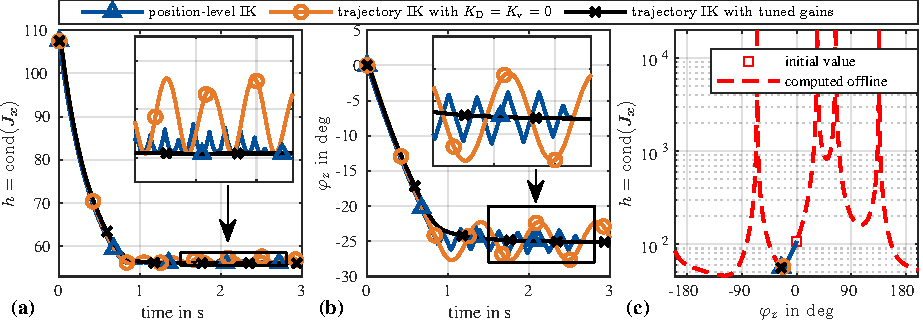
\includegraphics{figures/pkm_nullspace_case1_overview.pdf}
	\caption{Simulation results of the parallel robot starting in the non-singular pose from Fig~\ref{fig:pkm_poses}\,a.}
	\label{fig:pkm_results_from_nonsingular}
\end{figure*}

\section{\uppercase{Case Study}}
\label{sec:casestudy}


The validation of the nullspace projection of section~\ref{sec:parrob} and the controller scheme of section~\ref{sec:control_loop} is performed in the following via simulation.
The assumption of a five-DoF task and a six-DoF robot still holds.
A parallel robot is used since the benefits and applicability of the proposed methods are better than for serial robots.

\subsection{Singularity Avoidance in Nullspace}
\label{sec:casestudy_nullspace}

The nullspace motion is first examined without an additional robot task motion, i.e. $\dot{\bm{q}}_\mathrm{T}=\ddot{\bm{q}}_\mathrm{T}=\bm{0}$.
The presented method can be applied to optimize any scalar performance criterion $h$ in the nullspace of the task redundancy.
In this example, the condition number of the robot Jacobian matrix of (\ref{eq:par_jacobi_inv}) is selected as $h(\bm{q},\bm{x})=\mathrm{cond}(\bm{J}_{\bm{x}})=\mathrm{cond}(\bm{J}_{\bm{x}}^{-1})$.
Minimizing this criterion moves the manipulator towards low condition numbers and therefore away from singularities.

A hexapod parallel (Stewart-Gough type) robot is considered in a pose $\bm{y}$ with a high tilting angle of the platform.
Technical details of the robot are given in Table~\ref{tab:hexapod_values}.
The high tilting angle (expressed by $\varphi_x$ and $\varphi_y$) presents the general spatial case, where the representation of orientation by Cardan angles ($X$-$Y$'-$Z$'') is beneficial.
The torsion angle $\varphi_z$ of the platform is set to two different values, depicted in Fig~\ref{fig:pkm_poses}\,a and \ref{fig:pkm_poses}\,b, representing the two cases to be investigated.

\subsubsection{Case 1: Non-Singular Initial Pose}
\label{sec:eval_case1}

\begin{figure*}[tb]
	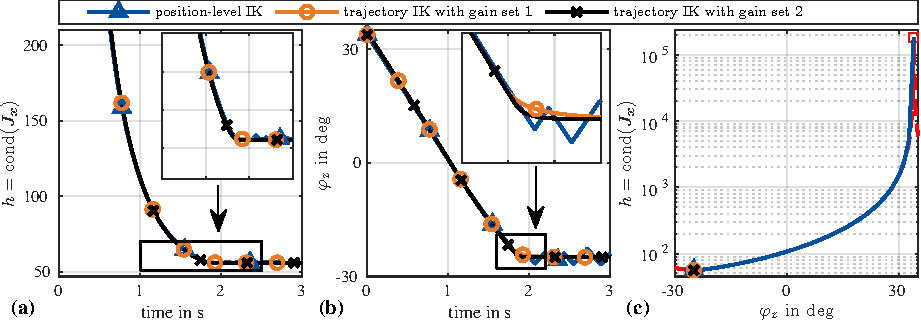
\includegraphics{figures/pkm_nullspace_case2_overview.pdf}
	\caption{Simulation results of the parallel robot starting in the singular pose from Fig~\ref{fig:pkm_poses}\,b.}
	\label{fig:pkm_results_from_singular}
\end{figure*}

In the first case the robot starts in the non-singular pose of Fig~\ref{fig:pkm_poses}\,a with $\varphi_{z,\mathrm{start},1}{=}$\SI{0}{\degree}.
The values of the optimization objective $h$ over the redundant coordinate $\varphi_z$ are depicted in Figure~\ref{fig:pkm_results_from_nonsingular}\,c over a full rotation of the platform (red dashed line).
The overall performance of the robot is highly influenced by singularities, which are located at $\varphi_{z,\mathrm{sing,1}}\,{\approx}\,$\SI{-65}{\degree}, $\varphi_{z,\mathrm{sing,2}}\,{\approx}\,$\SI{34}{\degree}, $\varphi_{z,\mathrm{sing,3}}\,{\approx}\,$\SI{64}{\degree} and $\varphi_{z,\mathrm{sing,4}}\,{\approx}\,$\SI{136}{\degree}.
The locations of these singularities $\varphi_{z,\mathrm{sing}}$ were obtained from global evaluation of the redundant coordinate.

The nullspace motion is first generated by the \emph{position-level IK scheme} of (\ref{eq:ser_position_ik}).
The convergence towards the next local minimum of $h(\varphi_{z,\mathrm{final}}){=}56.1$ at $\varphi_{z,\mathrm{final}}{=}$\SI{-25}{\degree} can be comprehended from Fig~\ref{fig:pkm_results_from_nonsingular}\,a for $h(t)$, from Fig~\ref{fig:pkm_results_from_nonsingular}\,b for $\varphi_z(t)$ and from Fig~\ref{fig:pkm_results_from_nonsingular}\,c for the characteristic diagram $h(\varphi_z)$ (blue lines).
Compared to the initial value of $h(\varphi_{z,\mathrm{start},1}){=}107.5$ it can be assumed that the overall performance of the robot is improved by the nullspace motion.
This could be quantified by other, more physically motivated performance criteria such as accuracy, stiffness or actuator forces, but is out of scope of this publication.
The position-level scheme only serves as a reference, since no time relation is included originally and the steps $k$ of (\ref{eq:ser_position_ik}) are transferred to a time basis $t$ using the joint velocity limits.
A $C^2$-continuous trajectory (with continuously differentiable position and velocity) regarding limits for $\dot{\bm{q}}$ and $\ddot{\bm{q}}$ can not be assured by this.

Therefore, the nullspace motion is obtained using the \emph{trajectory IK scheme} from (\ref{eq:par_nullspace_actjoint}) and section~\ref{sec:parrob_taskred_actspace} in the \emph{actuator space}.
To emphasize the argumentation of section~\ref{sec:control_loop}, first the feedback gains $K_\mathrm{D}=0$ and $K_\mathrm{v}=0$ are used with $K_\mathrm{P}=1$.
A discrete-time implementation with sample time \SI{1}{\milli\second} was used.
The time evolution in Fig~\ref{fig:pkm_results_from_nonsingular}\,a and \ref{fig:pkm_results_from_nonsingular}\,b shows undamped oscillations (orange lines).
Therefore this parameterization does not allow to reach the purpose of moving to the next local optimum of $h$ with little overshoot and fast convergence.
%
To accomplish this control objective, the parameterization $K_\mathrm{v}{=}0.5$, $K_\mathrm{P}{=}1$ and $K_\mathrm{D}{=}0.5$ is selected, which was obtained by manual tuning.
The motion controller now reaches the optimal value of $\varphi_{z,\mathrm{final}}{=}$\SI{-25}{\degree} within about two seconds (black lines).


\subsubsection{Case 2: Singular Initial Pose}
\label{sec:eval_case2}

The proposed new nullspace projection approach of the full joint coordinate space of (\ref{eq:par_nullspace_fulljoint}) and section~\ref{sec:parrob_taskred_fullspace} has to be used if the initial pose or an intermediate pose represents a singular configuration.
This is the case for the second starting pose $\varphi_{z,\mathrm{start},2}{=}$\SI{33.8}{\degree}, where a numeric value for the condition number of $\mathrm{cond}(\bm{J}_{\bm{x}}^{-1})=1.8 \cdot 10^5$ is reached.
In this case, the inversion of $\bm{J}_{\bm{x}}^{-1}$ is not possible (or at least does not produce feasible results).
Controller schemes relying on $\bm{J}_{\bm{x}}$, e.g. formulated in the operational space, would produce high accelerations or high actuator forces.
Therefore a controller scheme avoiding this drawback has to be used as a fallback to physically operate the robot, e.g. a scheme defined only in the actuator space.

The motion controller of section~\ref{sec:control_loop} is again used to generate the nullspace motion with singularity avoidance, as in the previous case.
This time, the motion is generated in the \emph{full joint space} from (\ref{eq:par_nullspace_fulljoint}) and section~\ref{sec:parrob_taskred_fullspace} with the \emph{trajectory IK scheme}.

\begin{figure*}[tb]
	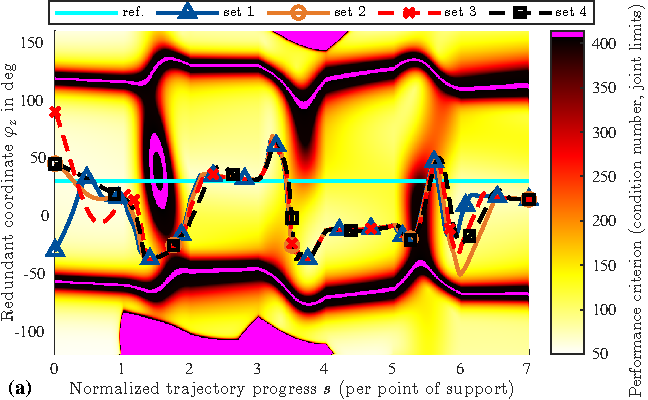
\includegraphics{nullspace_traj.pdf}
	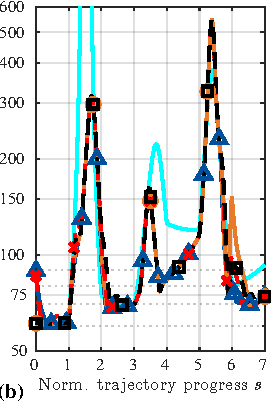
\includegraphics{nullspace_traj_condition.pdf}
	\caption{(a) Performance map of the condition number over the trajectory progress and all possibilities for the redundant coordinate. (b) Distribution of the condition number over the trajectory for different settings.}
	\label{fig:pkm_trajectory_results}
\end{figure*}

The simulation results are given in Fig~\ref{fig:pkm_results_from_singular}.
Again, the position-level IK and two parameterizations of the trajectory IK are shown, while the position-level IK only serves as comparison.
The gains for the trajectory IK were tuned manually and using a particle swarm optimization and were set to $K_\mathrm{v}{=}0.03$, $K_\mathrm{D}{=}0.01$, and $K_\mathrm{P}{=}0.05$ in the first set and $K_\mathrm{v}{=}0.2$, $K_\mathrm{D}{=}0.03$ and $K_\mathrm{P}{=}0.5$ in the second set.
With both sets again a fast convergence within two seconds can be achieved while maintaining the limits for $\bm{q}$, $\dot{\bm{q}}$ and $\ddot{\bm{q}}$.
The extent of oscillation and the settling time is influenced by the selected rather low joint velocity limits (see Table~\ref{tab:hexapod_values}).
This shows the feasibility of the proposed nullspace scheme in full joint coordinates to be able to leave a type-II singularity.
%
The gain values above are not directly comparable to the ones of section~\ref{sec:eval_case1}, since there the compensation of the term $k(\bm{q})$ of (\ref{eq:par_nullspace_relation}) is attempted.
The values in section~\ref{sec:eval_case1} are divided by $k'(\bm{q},\bm{x})=||\tilde{\bm{J}}^{-1}_{\bm{x}} \bm{J}_{\bm{x}}||$, which presents a rough estimate.
The determination of the exact relation is subject of ongoing work.
Also, a general rule to determine the controller gains has to be found.


\begin{figure}[b]
	\input{./figures/pkm_traj_start_pose.pdf_tex}
	\caption{Starting pose of the robot trajectory for $\varphi_z{=}0$.}
	\label{fig:pkm_trajectory_startpose}
\end{figure}

\subsection{Trajectory with Singularity Avoidance}
\label{sec:casestudy_traj}

The previous evaluation of section~\ref{sec:casestudy_nullspace} shows the general property of the task coordinate's nullspace to allow moving the manipulator away from singularities without an additional task motion.
In a practical application like milling a pointing task trajectory $\bm{y}(t)$ with $C^2$ differentiability (or higher) is given.
Therefore a task trajectory $\ddot{\bm{q}}_\mathrm{T}(t)$ 
according to (\ref{eq:par_ik_acc_taskspace}) is active in the motion generation scheme summarized in Figure~\ref{fig:control_loop}.
Since milling presents one of the major use cases of hexapod parallel robots, an exemplary trajectory of milling a \SI{45}{\degree} bezel to a rectangular pocket is used for evaluation, as visualized in Figure~\ref{fig:pkm_trajectory_startpose}.
The red, green and blue axes around the rectangle represent the $x$-, $y$- and $z$-axis of the end effector frame for $\varphi_z{=}0$.
Due to the task symmetry, only the pointing direction of the blue $z$-axes has to be aligned.
The tilting angle of \SI{45}{\degree} poses high requirements on the robot and emphasizes the necessity of an appropriate spatial orientation representation.
%The previous robot example is modified to accomplish a valid trajectory execution.
The trajectory is put together by rest-to-rest motions between eight poses $\bm{y}_i$ as points of support, summarized in Table~\ref{tab:trajectory_points} and corresponding to $s\,{=}\,0$ to $s\,{=}\,7$ in Figure~\ref{fig:pkm_trajectory_startpose}.
At each corner of the \SI{250}{\milli\metre}$\times$\SI{200}{\milli\metre}-rectangle a change of orientation is necessary to adjust the \SI{45}{\degree} angle for the next edge, corresponding to $1{\leq}s{\leq}2$, $3{\leq}s{\leq}4$ and $5{\leq}s{\leq}6$ in Figure~\ref{fig:pkm_trajectory_startpose}.
A normalized trajectory coordinate $s$ instead of the time $t$ is used to represent progress along the path in the figures of this section for the sake of simplicity.
Each rest-to-rest motion is assigned a range of one in $s$.
However, the trajectory is generated by a trapezoidal acceleration  profile ($C^2$ time-differentiable S-curve) with  $\dot{r}_{\mathrm{max}}{=}$\SI{50}{\milli\metre\per\second}, $\dot{\varphi}_{\mathrm{max}}{=}$\SI{10}{\degree}/s, a discrete sample time of \SI{1}{\milli\second} and acceleration and jerk times of \SI{10}{\milli\second}.
The duration of the trajectory is \SI{63.1}{\second}.

The global distribution of the condition number $h(\bm{q},\bm{x})=\mathrm{cond}(\bm{J}_{\bm{x}})$ is shown as a performance map in Figure~\ref{fig:pkm_trajectory_results} for the complete trajectory, represented by 1062 samples of the path coordinate $s$ on the horizontal axis. % from the variable X_tref (or s_ref) in ParRob_nullspace_trajectory.m
The vertical axis is chosen as the redundant coordinate $\varphi_z$ which was discretized in 361 samples in the range of ${\pm}$\SI{180}{\degree}. % these numbers come from the variable phiz_range in ParRob_nullspace_trajectory.m
The condition number is coded by the color of the map.
High condition numbers $h>400$ are saturated in the color code to dark red.
Singularities, which are defined as condition numbers $h>10^4$, and areas of joint limit violation are marked with magenta.
Creating the colored performance map in this resolution requires 383 thousand evaluations of the inverse kinematics and the performance criterion.
With this map a \emph{global optimization} of the coordinate $\varphi_z(s)$ can be performed, which corresponds to the methods of the state of the art.

Using a \emph{local optimization} on the contrary does not require the expensive computation of the performance map.
The nullspace motion of the redundant coordinate $\varphi_z$ is performed again by the nullspace controller scheme of section~\ref{sec:control_loop}.
Different settings for the nullspace controller are chosen for illustration and the resulting nullspace motion is shown as different lines in the performance map in Figure~\ref{fig:pkm_trajectory_results}\,a and as the evolution of the condition number over the progress of the trajectory in Figure~\ref{fig:pkm_trajectory_results}\,b.
The settings are listed in Table~\ref{tab:trajectory_ik_settings}.
Using different starting values and settings emphasizes the robustness of the approach.

It has to be mentioned that the effects of the nullspace gains are limited by the velocity and acceleration limits of the joints (see Table~\ref{tab:hexapod_values}).
%
Therefore mainly in the last part of the trajectory a difference between the settings becomes visible.
The overall behavior of avoiding areas of singularity is achieved with all settings.
The reference is a constant rotation of the platform with $\varphi_z{=}$\SI{30}{\degree} (cyan line in Figure~\ref{fig:pkm_trajectory_results}).
This presents a good solution at the beginning, but leads to a singularity during change of orientation at the second corner for $1\,{\leq}\,s\,{\leq}\,2$.

The first nullspace setting (set 1) in Figure~\ref{fig:pkm_trajectory_results} corresponds to the first setting in section~\ref{sec:eval_case2}.
The other settings each have different gains.
All nullspace settings produce a motion that avoids the first area of singularity at $s\,{\approx}\,1.5$.
Also a second area of high, but non-singular condition numbers at $s\,{\approx}\,3.7$ is avoided.
A third area of high condition numbers at $s\,{\approx}\,5.4$ can not be avoided, since the shape of the performance map leads to a dead end at the previous section of low condition numbers at $s\,{>}\,5$.
Here the disadvantage of the local optimization becomes apparent and a global optimization or a component of looking ahead (for higher $s$) would outperform the proposed approach.
The qualitative effect of the decreasing gains and increasing damping over the settings numbers can be seen at parts of the trajectory where a reconfiguration of the platform orientation is performed, e.g. at $s\,{\approx}\,2.1$ and $s\,{\approx}\,5.9$.
For lower gains the optimal platform rotation is achieved later (in the sense of time $t$ and therefore also of trajectory progress $s$).


\subsection{Evaluation of Computation Time}
\label{sec:eval_comptime}

The number of function evaluations required for the determination of the gradients of performance objectives obviously influences the computation time.
The inverse kinematics algorithms on position and trajectory level were implemented in \textsc{Matlab} as compiled stand-alone functions (using the \textsc{Matlab} code generator and mex files).
This combines fast iterations and efficient debugging with the \textsc{Matlab} graphical user interface on the one hand and fast runtime of \texttt{C++} code on the other hand.
The computation time was evaluated on a standard desktop computer (Intel Core i5-7500 CPU, \SI{3.40}{\giga\hertz}, Linux operating system, generic kernel, no real-time).
The hardware performance corresponds to typical PC-based robot controllers.
Measured computation times should be regarded relative to each other and in their order of magnitude and may differ on other computing hardware.

% Info: Timing numbers are printed in the Matlab scripts with enabled option usr_test_timing
% Timing is given after output of ParRob_nullspace_static_pose.m:
% * Timing Evaluation of position-level kinematics
Executing the \emph{position-level IK} in the evaluation of section~\ref{sec:casestudy_nullspace} requires 394 steps with the Newton-Raphson algorithm to compute an optimal pose which takes a mean computation time of \SI{226}{\milli\second} ($n{=}50$, $\sigma{=}$\SI{3.96}{\milli\second}).
The mean time per iteration is \SI{0.57}{\milli\second} ($\sigma{=}$\SI{0.01}{\milli\second}).
This corresponds to the blue lines in Figure~\ref{fig:pkm_results_from_nonsingular}.
555 iterations are necessary in section~\ref{sec:eval_case2}  with a similar mean time per iteration of \SI{0.56}{\milli\second} ($n{=}50$, $\sigma{=}$\SI{0.01}{\milli\second}, blue lines in Figure~\ref{fig:pkm_results_from_singular}).

% Timing is given after output of ParRob_nullspace_static_pose.m:
% * Timing Evaluation of position-level kinematics without using efficient form of gradient approximation
If a variation in all joint coordinates is computed separately according to section~\ref{sec:parrob_taskred_general}, one iteration takes \SI{1.78}{\milli\second} ($n{=}50$, $\sigma{=}$\SI{0.04}{\milli\second}). % or \SI{1.78}{\milli\second} (second case, $n{=}50$, $\sigma{=}$\SI{0.03}{\milli\second}).
Despite this method being not applicable to the case of section~\ref{sec:casestudy_nullspace}, this shows the significance of using the gradient computation by the  redundant coordinate's difference quotient from  section~\ref{sec:parrob_taskred_fullspace}.

% Timing is given after output of ParRob_nullspace_static_pose.m:
% * Timing Evaluation of trajectory kinematics
The computation of the null space motion in the actuation space according to section~\ref{sec:parrob_taskred_actspace} (and \ref{sec:eval_case1}) instead of the full joint space of section~\ref{sec:parrob_taskred_fullspace} (and \ref{sec:eval_case2}) does not improve the computation time of the \emph{trajectory IK} as expected in the current implementation.
A simulated time of \SI{10}{\second} and therefore 10,000 samples were computed to obtain the black and orange lines in Figures \ref{fig:pkm_results_from_nonsingular} and \ref{fig:pkm_results_from_singular}.
Timing evaluation was performed with $n{=}50$ repetitions.
In the actuated joint space (Figure~\ref{fig:pkm_results_from_nonsingular}) the computation time was \SI{9.3}{\second} ($\sigma{=}$\SI{52}{\milli\second}, orange line, \SI{0.93}{\milli\second} per sample) and \SI{9.7}{\second} ($\sigma{=}$\SI{243}{\milli\second}, black line).
In the full joint space (Figure~\ref{fig:pkm_results_from_singular}) the computation times were \SI{9.1}{\second} ($\sigma{=}$\SI{147}{\milli\second}, orange line) and \SI{9.2}{\second} ($\sigma{=}$\SI{15}{\milli\second}, black line).
Using the \textsc{Matlab} profiler on the non-compiled function reveals that computing $\bm{N}_{\bm{q}}$ of section~\ref{sec:parrob_taskred_fullspace} only takes about \SI{3.5}{\percent} of the total time and $\bm{N}_{\bm{\theta}}$ of section~\ref{sec:parrob_taskred_actspace} only takes about \SI{0.6}{\percent} of the total time.
Performing the $6 \times 6$ inverse necessary for the latter approach only takes \SI{0.15}{\percent}.
The term $\bm{N}_{\bm{q}}$ is also used for a nullspace motion upon joint position limit violation and is computed in all cases.
This explains the higher computation times in the latter cases.
Due to the small differences between the computation times the full coordinate space (section~\ref{sec:parrob_taskred_fullspace}) should always be used within the current implementation of the algorithm.


% Timing is given after output of ParRob_nullspace_trajectory.m:
% * Timing Evaluation of trajectory inverse kinematics
The effort for computing the nullspace motion in general becomes visible when comparing the non-redundant case in section~\ref{sec:casestudy_traj} (cyan line in Figure~\ref{fig:pkm_trajectory_results}) to the redundant cases (other lines).
The non-redundant trajectory takes \SI{12.7}{\second} ($n{=}10$, $\sigma{=}$\SI{23}{\milli\second}, \SI{0.20}{\milli\second} per sample) while the redundant case takes \SI{54.7}{\second} ($n{=}10$, $\sigma{=}$\SI{139}{\milli\second}, \SI{0.87}{\milli\second} per sample).

In summary it can be stated that despite the higher computational effort for the nullspace motion algorithms already the current implementation can be used as an online controller, since the runtime stays below \SI{1}{\milli\second}, which is the typical control loop sample time for such robots.
The \textsc{Matlab} functions can be directly used as blocks in \textsc{Simulink} which can be deployed with the EtherLab toolchain (using standard Ethernet hardware of a desktop computer with Linux realtime kernel as target and the EtherCAT bus as sensor/actuator interface).
Runtime may further be improved by disabling computations with little effect and by using functions specific to the robot instead of the currently used general approach without limiting assumptions.


\section{\uppercase{Conclusions and Outlook}}
\label{sec:conclusion}

A simplified computation of the gradients of performance criteria of robot manipulators is presented, which exploits the properties of task redundancy of degree one.
This presents an extension to the application of redundancy resolution frameworks for serial and parallel robot manipulators.
The performance criteria have to be evaluated under real-time conditions to allow their online optimization.
Therefore, deployment of more sophisticated performance criteria will be possible by reducing the number of function evaluations necessary for gradient calculation.

With the presented nullspace formulation avoiding singularities for parallel robots is possible by performing the calculations in the full joint space.
Using this more complex model allows to define a fallback controller for exiting a singularity of type II.
This can be used if tracking a trajectory fails due to external disturbance or in case of manually guiding a parallel robot platform in teaching mode.
In offline trajectory planning such as for machining tasks the method can be used to locally optimize path segments combined with global optimization of the whole path similar to Figure~\ref{fig:pkm_trajectory_results} of the paper.

Compared to the authors' earlier work, the redundancy resolution schemes of \cite{KotlarskiDoHeiOrt2010} are extended for an efficient continuous adaption of a redundant degree of freedom instead of the previously favored discrete optimization.
The need for computationally expensive global optimization decreases.
The theoretical contribution \cite{SchapplerTapOrt2019} regarding kinematic modeling is brought one step closer towards an application.

Future work comprises finding rules for setting gain parameters of the nullspace scheme, finding the analytic relation (\ref{eq:par_nullspace_relation}) between nullspace projectors of parallel robot actuator space and full joint space, and performing a stability analysis using control theory. % profound

\vspace{0.2cm} % push tables down in the column

\begin{table}[hb] % see Matlab script
	\caption{Characteristic values of the parallel robot of Sec.~\ref{sec:casestudy}}
	\label{tab:hexapod_values}
	\centering
	\setlength\tabcolsep{3 pt}
	\begin{tabular}[t]{|c|c|c|c|}
		\hline
		\textbf{Name} & \textbf{Symbol} & \textbf{Value} & \textbf{Unit} \\
		\hline
		base diameter & $d_\mathrm{B}$ & 1200 &mm \\
		platform diam. & $d_\mathrm{P}$ & 400 & mm \\ %  (Sec.\,\ref{sec:casestudy_nullspace})
		(in Sec.\,\ref{sec:casestudy_traj}) & $d_\mathrm{P}$ & 300 & mm \\
		joint pair distance & $d_\mathrm{J}$ & 100 & mm \\
		platform position & $r_x$, $r_y$, $r_z$ & 50, 30, 600 & mm \\
		platf. orientation & $\varphi_x, \varphi_y$ & $30^\circ,{-}30^\circ$ & deg \\
		act. j. stroke limits & $\theta_{i,\mathrm{min/max}}$ & 600, 1200 & mm\\ % \SI{600}{\milli\metre}, \SI{1200}{\milli\metre} % ,$\theta_{i,\mathrm{max}}$
		pass j. angle lim. & --- & not set & \SI{}{deg}\\
		act. j. velo. limits & $\dot{\theta}_{i,\mathrm{max}}$ & 2 & \SI{}{\metre\per\second} \\
		pass j. velo. lim. & --- & 45 & \SI{}{deg\per\second}\\
		act. j. acc. limits & $\ddot{\theta}_{i,\mathrm{max}}$ & 20 & \SI{}{\metre\per\square\second} \\
		pass j. acc. lim. & --- & 1146 & \SI{}{deg\per\second\square}\\
		\hline
	\end{tabular}
\end{table}

\begin{table}[hb]
	\caption{Rest poses $\bm{y}_i$ of the trajectory in Figures~\ref{fig:pkm_trajectory_results} and \ref{fig:pkm_trajectory_startpose}}
	\label{tab:trajectory_points}
	\centering
	\begin{tabular}[t]{|c|c|c|c|c|c|}
		\hline
		$s$ & $r_x$ & $r_y$ & $r_z$ & $\varphi_x$ & $\varphi_y$ \\
		& mm & mm & mm & deg & deg \\
		\hline
		0 & -50 & 40 & 700 & 45 & 0\\
		1 & 200 & 40 & 700 & 45 & 0\\
		2 & 200 & 40 & 700 & 0 & -45\\
		3 & 200 & -160 & 700 & 0 & -45\\
		4 & 200 & -160 & 700 & -45 & 0\\
		5 & -50 & -160 & 700 & -45 & 0\\
		6 & -50 & -160 & 700 & 0 & 45\\
		7 & -50 & 40 & 700 & 0 & 45\\
		\hline
	\end{tabular}
\end{table}
\begin{table}[b]
	\caption{Settings for the nullspace motion  of the trajectory in Figure~\ref{fig:pkm_trajectory_results} and Figure~\ref{fig:pkm_trajectory_startpose}}
	\label{tab:trajectory_ik_settings}
	\centering
	\begin{tabular}[t]{|c|c|c|c|c|c|}
		\hline
		Param. & ref. & set 1 & set 2 & set 3 & set 4 \\
		\hline
		$\varphi_{z,0}$ & \SI{30}{\degree} & \SI{-30}{\degree} & \SI{45}{\degree} & \SI{90}{\degree} & \SI{45}{\degree}\\
		$K_\mathrm{v}$ & --- & 0.03 & 0.1 & 0.25 & 0.5\\
		$K_\mathrm{P}$ & --- & 0.05 & 0.01 & 0.005 & 0.0025\\
		$K_\mathrm{D}$ & --- & 0.01 & 0.002 & 0.001 & 0.0005\\
		\hline
	\end{tabular}
\end{table}

\newpage % to have ack.+ref. on last page

\section*{\uppercase{Acknowledgements}}

The authors acknowledge the support by the Deutsche Forschungsgemeinschaft (DFG) under grant number 341489206.
\textsc{Matlab} Code to reproduce the results is available at GitHub under free license at https://\\\url{github.com/SchapplM/robotics-paper_icinco2021}.

\bibliographystyle{apalike}
{\small
\bibliography{references}}


\end{document}

